
%\documentclass[mathserif]{beamer}
\documentclass[handout]{beamer}
%\usetheme{Goettingen}
%\usetheme{Warsaw}
\usetheme{Singapore}



%\usetheme{Frankfurt}
%\usetheme{Copenhagen}
%\usetheme{Szeged}
%\usetheme{Montpellier}
%\usetheme{CambridgeUS}
%\usecolortheme{}
%\setbeamercovered{transparent}
\usepackage[english, activeacute]{babel}
\usepackage[utf8]{inputenc}
\usepackage{amsmath, amssymb}
\usepackage{dsfont}
\usepackage{graphics}
\usepackage{cases}
\usepackage{graphicx}
\usepackage{pgf}
\usepackage{epsfig}
\usepackage{amssymb}
\usepackage{multirow}	
\usepackage{amstext}
\usepackage[ruled,vlined,lined]{algorithm2e}
\usepackage{amsmath}
\usepackage{epic}
\usepackage{epsfig}
\usepackage{fontenc}
\usepackage{framed,color}
\usepackage{palatino, url, multicol}
%\algsetup{indent=2em}
\newcommand{\factorial}{\ensuremath{\mbox{\sc Factorial}}}
\newcommand{\BIGOP}[1]{\mathop{\mathchoice%
{\raise-0.22em\hbox{\huge $#1$}}%
{\raise-0.05em\hbox{\Large $#1$}}{\hbox{\large $#1$}}{#1}}}
\newcommand{\bigtimes}{\BIGOP{\times}}
\vspace{-0.5cm}
\title{Natural Language Processing \\ Vectors Space Model and Information Retrieval}
\vspace{-0.5cm}
\author[Felipe Bravo Márquez]{\footnotesize
%\author{\footnotesize  
 \textcolor[rgb]{0.00,0.00,1.00}{Felipe Bravo-Marquez}} 
  
 

\date{\today}

\begin{document}
\begin{frame}
\titlepage


\end{frame}

\begin{frame}\frametitle{Motivation}


  \begin{itemize}
   \item How does a search engine such as Duckduckgo or Google retrieve relevant documents from a given query?
   \item How can a company process the claims left by its users on its Web portals?
  \end{itemize}

The following areas of knowledge study these problems:

\begin{itemize}
 \item \emph{Information Retrieval}:  science of searching for information in a documents.
 \item \emph{Text Mining}: Extraction of knowledge from text.
\end{itemize}

Both of them are closely related to NLP! (the borders between these fields are unclear)

\end{frame}

\begin{frame}\frametitle{Tokens and Types}
{\footnotesize
Tokenization: The task of splitting a sentence or document into \emph{tokens}. \\
Additional transformations can be employed such as the removal of special characters (e.g., punctuation), lowercasing, etc. ~\cite{manning2008}. 

\begin{block}{Example}
Input: I like human languages and programming languages.\\
Tokens: [I] [like] [human] [languages] [and] [programming] [languages]
\end{block}

A \emph{type} is a class of \emph{token} containing a single sequence of characters.
They are obtained by identifying unique tokens within the document.

\begin{block}{Types}
Tipos: [I] [like] [human] [languages] [and] [programming]  \\
\center{\textit{The token \emph{languages} was repeated in the sentece}}
\end{block}



 }
\end{frame}

\begin{frame}\frametitle{Vocabulary Extraction }
\footnotesize{
A  \emph{term} is a normalized \emph{type}. The vocabulary $V$, is the set of terms (normalized unique tokens) within a collection of documents or corpus $D$.
 
\begin{block}{Stopwords removal}
\begin{itemize}
 \item In order to reduce the size of the vocabulary and eliminate terms that do not provide much information, terms that occur with high frequency are in the corpus are elminated. 
 \item These terms are called \emph{stopwords} and include  articles, pronouns, prepositions and conjunctions. \\
Example: [a, an, and, any, has, do, don't, did, the, on].\footnote{Related concepts: function words, closed-class words.}
\end{itemize}

The removal of stopwords can be inconvenient in many NLP tasks!! 
\\ Example: I don't like pizza $=>$ pizza  ( ``I'', ``don't'', and ``like'' were removed)

\end{block}


}
 
\end{frame}


\begin{frame}\frametitle{Stemming}
\footnotesize{
A process in which terms are transformed to their root in order to reduce the size of the vocabulary. It is carried out on the basis of a set of word reduction rules. \\ Example: Porter's Algorithm.

\begin{figure}[h!]
	\centering
	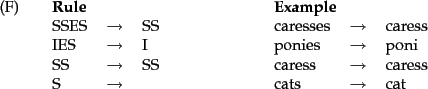
\includegraphics[scale=0.45]{pics/porter.png}
\end{figure}

 Example: $d$ = I like human languages and programming languages $=>$
I like human languag and program languag \footnote{\url{http://9ol.es/porter_js_demo.html}}

The vocabulary of document $d$ after removing stopwords and performing stemming:


\begin{table}
\centering
\begin{tabular}{c|c}
\hline
termId & value \\ 
\hline
t1 & human \\ 
t2 & languag \\ 
t3 & program\\ 
\hline
\end{tabular}
\end{table}

}
 
\end{frame}


\begin{frame}\frametitle{Lemmatization}
\footnotesize{

\begin{itemize}
 \item Another strategy to transform words to their root. It performs a morphological analysis using reference dictionaries (lookup tables) to create equivalence classes between \emph{types}.
\item For example for the token \emph{saw}, a stemming rule could return the term \emph{s}, while through lemmatization a dictionary would give us \emph{see}. 

\end{itemize}





}
\end{frame}



\begin{frame}\frametitle{Zipf's law [1]}
\footnotesize{
\begin{itemize}
\item The Zipf's law, proposed by \emph{George Kingsley Zipf} in \cite{zipf1935}, is an empirical law about the frequency of terms within a collection of documents (corpus). 
\item It states that the frequency $f$ of a term in a corpus is inversely proportional to its $r$ ranking in a sorted frequency table:
\begin{equation}
	f = \frac{cf}{r^{\beta}}
\end{equation}
\item Where $cf$ is a constant dependent on the collection and $\beta > 0$ is a decay factor.
\item If $\beta = 1$, then $f$ follows exactly Zipf's law, otherwise it follows a Zipf-like distribution. 

\item The law relates to the principle of minimum effort. We often use a few words to write ideas.

\item The Zipf law is a type of power law distribution (long tail distributions)


\end{itemize}


}
 
\end{frame}


\begin{frame}\frametitle{Zipf's law [2]}
\footnotesize{

\begin{figure}[h!]
	\centering
	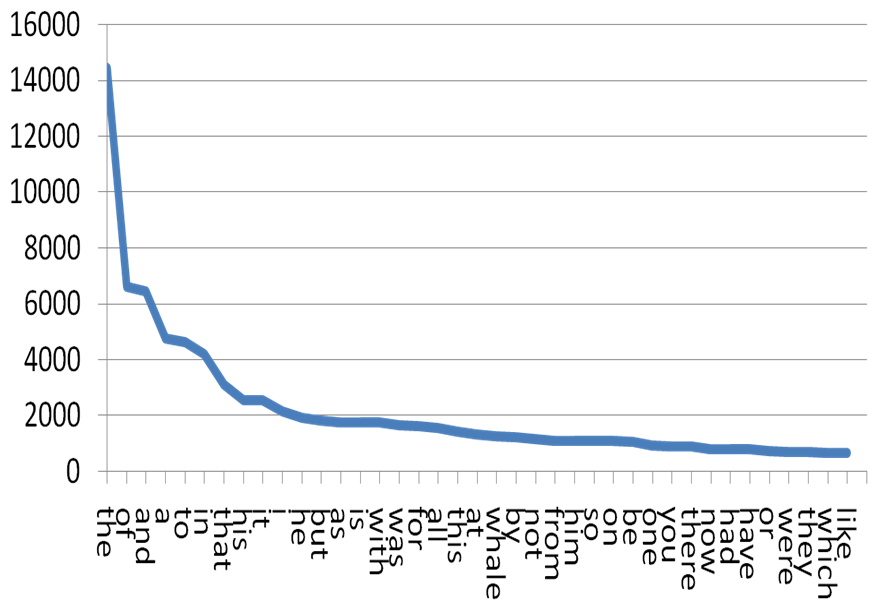
\includegraphics[scale=0.5]{pics/zipf1.png}
	\caption{Zipf's law}
\end{figure}
\begin{itemize}
 \item If we plot a $log-log$ graph, we obtain a straight line with slope  $-\beta^{-1}$.
 \item Most frequent words can be used to buil a \emph{stopwords} list. 
\end{itemize}
}



 
\end{frame}

\begin{frame}\frametitle{Posting List and Inverted Index}
{\footnotesize Let $D$ be a collection of documents  and $V$ the vocabulary of all terms extracted from the collection:

\begin{itemize}
 \item The posting list of a term is the list of all documents where the term appears at least once.
 \item An inverted index is a dictionary-type data structure mapping terms $t_{i} \in V$ into their corresponding posting lists.  ddf
 \begin{displaymath}
  <term> \rightarrow <docId>^*
 \end{displaymath}

\end{itemize}

\begin{figure}[h!]
	\centering
	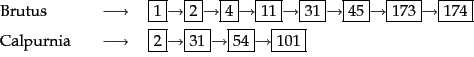
\includegraphics[scale=0.6]{pics/invFile.png}
	\caption{Inverted Index}
\end{figure}



}
\end{frame}



\begin{frame}\frametitle{Web Search Engines [1]}


{\footnotesize
  A search engine is an information retrieval system designed for searching information on the Web (solving information needs) \cite{manning2008}. Its basic components are:  

\begin{block}


\begin{itemize}
\item Crawler: a robot that navigates the Web according to a defined strategy. It usually starts by browsing a set of seed websites and continues to browse their hyperlinks.
\item Indexer: in charge of maintaining an inverted index with the content of the pages traversed by the Crawler.
\item Query processor: in charge of processing user queries and searching the index for the documents most relevant to a query.
\item Ranking function: the function used by the query processor to rank documents indexed in the collection by relevance according to a query.
\item User interface: receives the query as input and returns the documents ranked by relevancy.
\end{itemize}

\end{block}
}

\end{frame}


\begin{frame}\frametitle{Web Search Engines [2]}

\begin{figure}[h!]
	\centering
	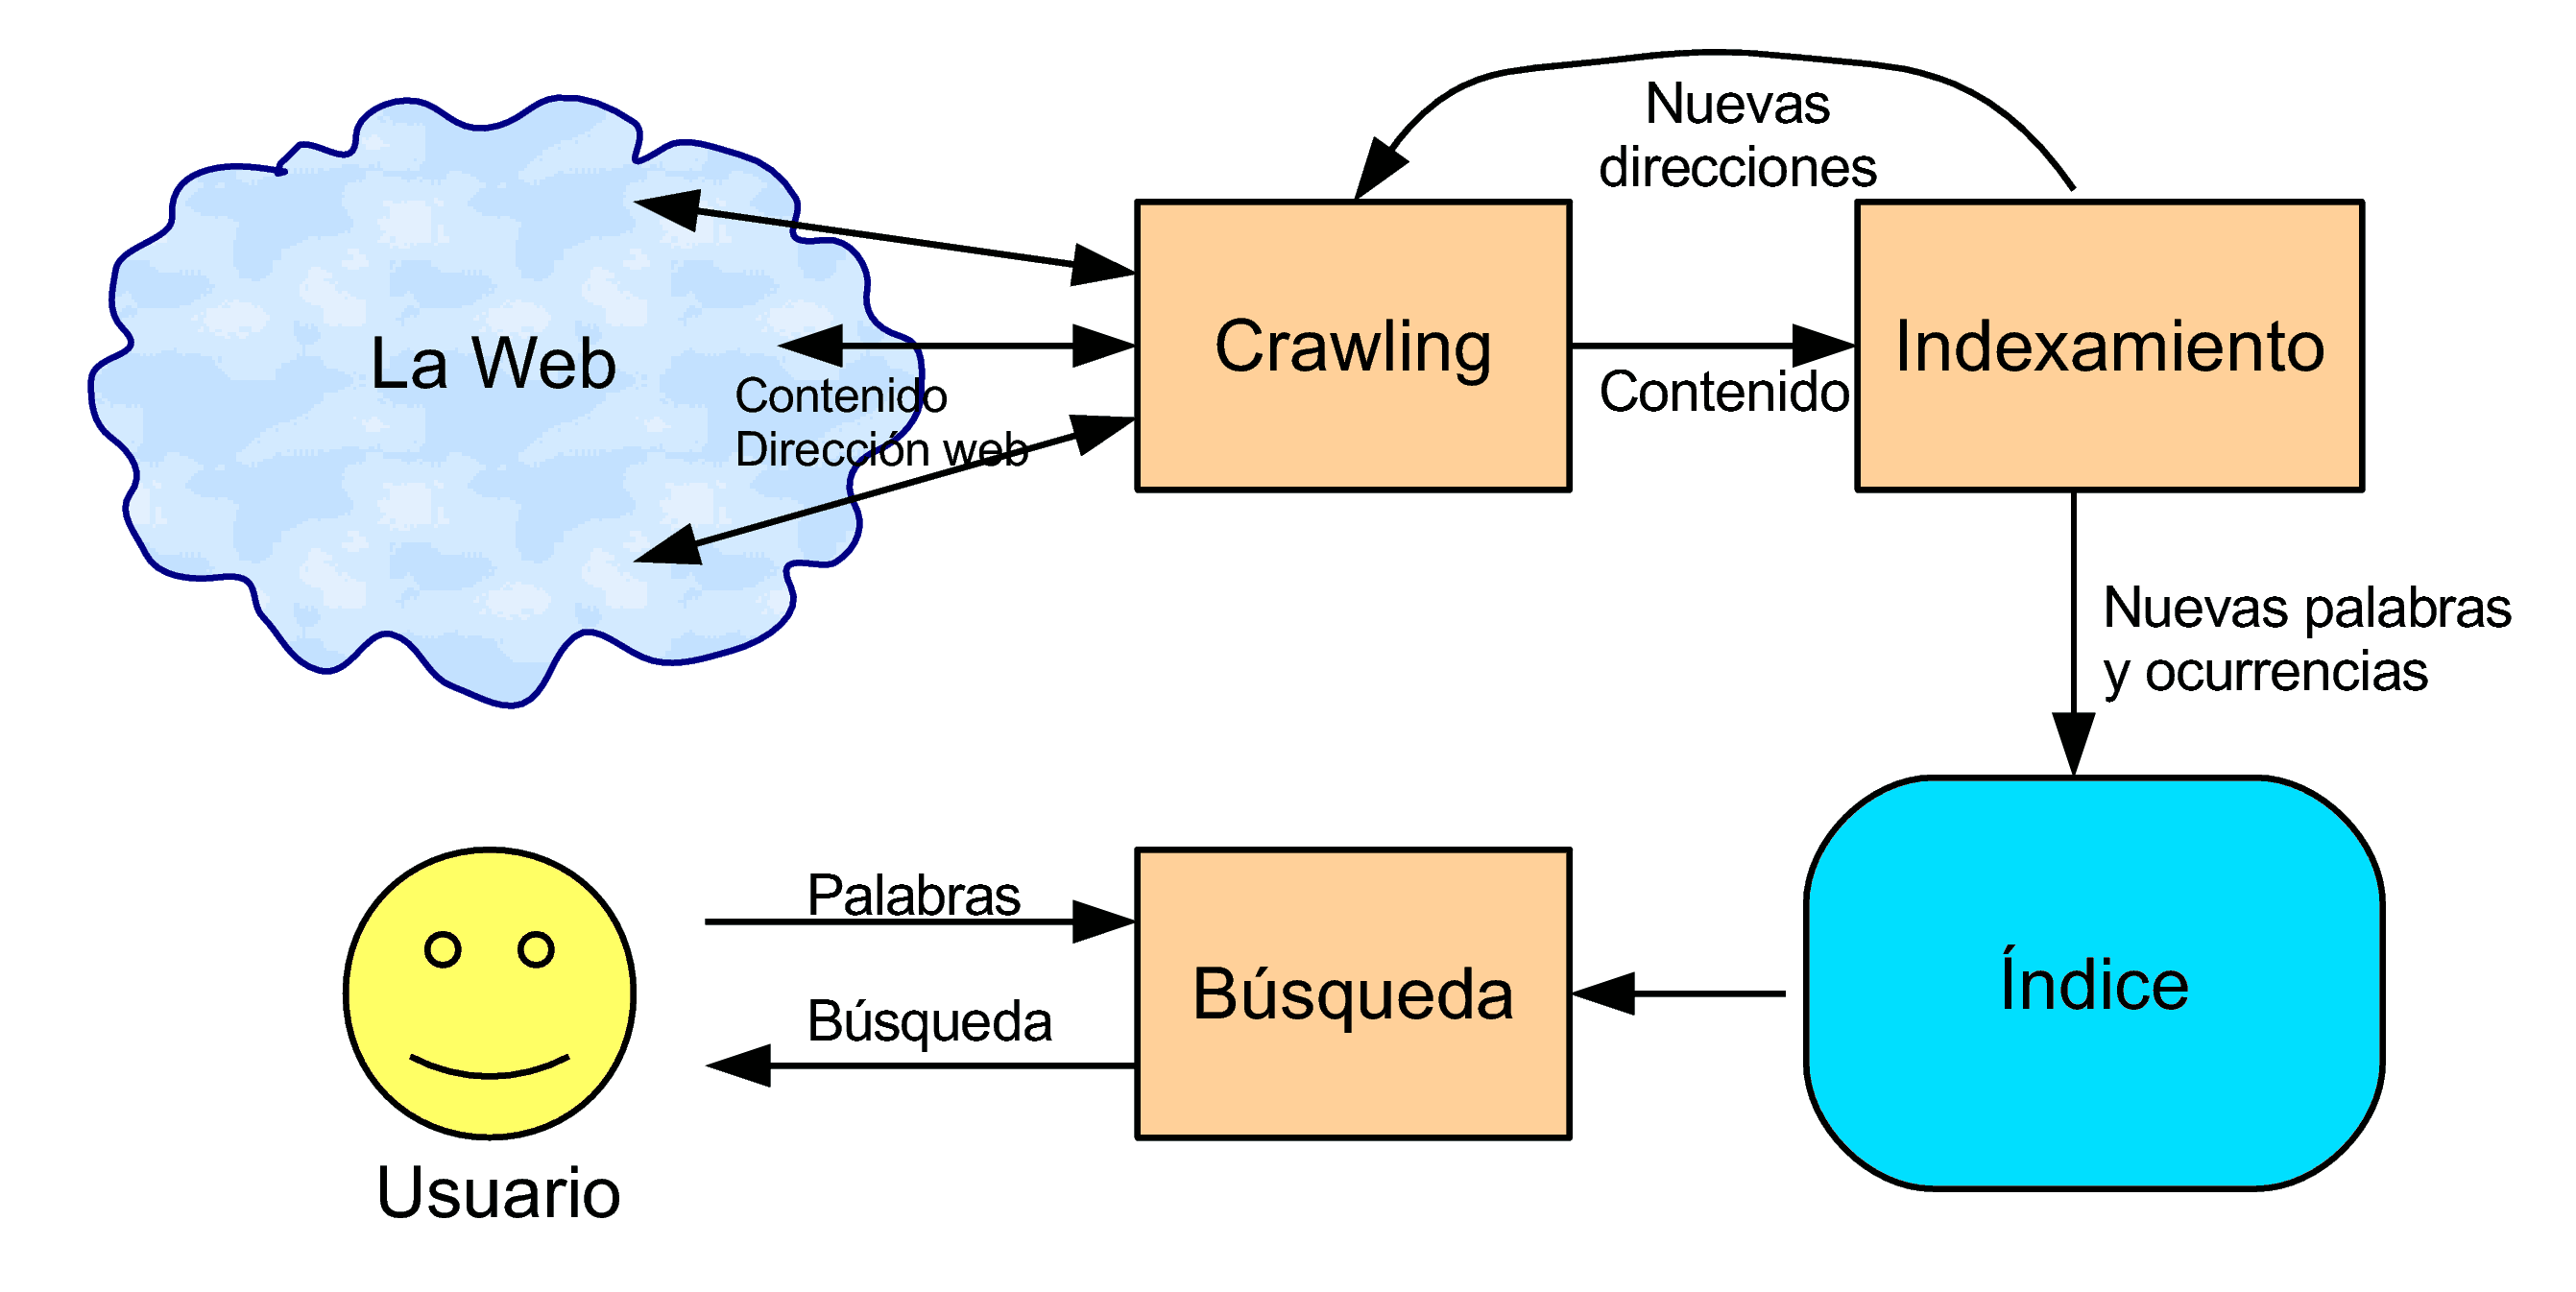
\includegraphics[scale=0.25]{pics/searchengine.png}
	\caption{ The various components of a web search engine~\cite{manning2008}.}
\end{figure}

\end{frame}

\begin{frame}\frametitle{Vector Space Models}
\footnotesize{
\begin{itemize}
 \item Para poder rankear las consultas, o medir la similitud entre dos documentos necesitamos una métrica de similitud.
 \item Representamos los documentos como vectores de términos, donde cada término es una dimensión.
 \item A este tipos de modelos se le llame \emph{Bag of Words}. Perdemos el orden de las palabras. 
 \item El valor de cada dimensión, es un peso que representa la relevancia del término $t_{i}$ en el documento $d$.

\begin{equation}
 d_{j} \rightarrow \overrightarrow{d_{j}}=(w(t_{1},d_{j}),...,w(t_{|V|},d_{j}))
\end{equation}

\item ¿Cómo podemos modelar el aporte de información de un término en un documento?
 
\end{itemize}

}
 
\end{frame}

\begin{frame}\frametitle{Term Frequency - Inverted Document Frequency [1]}
\footnotesize{
\begin{itemize}
 \item Se define $Tf_{i,j}$, como la frecuencia del término $t_{i}$ en el documento $d_{j}$.
 \item Un término que aparece $10$ veces debiese aportar mayor información que uno aparece una vez.
 \item ¿Qué pasa cuando tenemos documentos muchos más largos que otros?
 \item Podemos normalizar por la frecuencia máxima de término en el documento. 
\begin{displaymath}
 Tf_{i,j}=\frac{f_{i,j}}{max \ f_{i,j}}
\end{displaymath}
\item ¿Un término que aparece en muy pocos documentos aporta más o menos información que uno que aparece varias veces?
\item Por ejemplo, el documento \emph{El señor alcalde de Malloco}. El término \emph{Malloco} aparece en menos documentos que \emph{alcalde}, por lo que debiese ser más descriptivo. 
\end{itemize}


} 
\end{frame}

\begin{frame}\frametitle{Term Frequency - Inverted Document Frequency [2]}
\footnotesize{ 
\begin{itemize}
 \item Sea $N$ el número de documentos en la colección y $n_{i}$ el número de documentos donde aparece el término $t_{i}$, se define el $idf$ del término $t_{i}$ como: 
 \begin{displaymath}
  idf_{t_{i}}= log_{10}(\frac{N}{n_{i}})
 \end{displaymath}
\item Un término que aparece en todos los documentos tendría $idf=0$ y uno que aparece en el $10\%$ de la colección tendría $idf=1$.

\item El modelo de score $Tf-idf$ combina ambos modelos, quedando el peso $w$ de un término sobre un documento como:
\begin{displaymath}
w(t_{i},d_{j})=Tf_{i}\times log_{10}(\frac{N}{n_{i}}) 
\end{displaymath}

\item Las consultas a un motor de búsqueda también pueden modelarse como vectores, pero las consultas tienen en promedio entre $2$ y $3$ términos. Para evitar tener tantas dimensiones nulas, se usa un factor de suavizamiento en el vector:
\begin{displaymath}
 w(t_{i},d_{j})=(0.5+0.5\times Tf_{i,j})log_{10}(\frac{N}{n_{i}}) 
\end{displaymath}



\end{itemize}



}

\end{frame}

\begin{frame}\frametitle{Similarity between Vectors}
\footnotesize{
\begin{itemize}
 \item Una vez representados, los documentos y consultas como vectores, podemos medir su similitud.
 \item Una alternativa sería usar la distancia euclidiana, pero la variabilidad de largo entre documentos afectaría a la métrica.
 \item Lo más usado es usar el coseno del ángulo entre los vectores como medida de similitud.
 \item Si los documentos son iguales, el ángulo vale $0$ y el coseno $1$. En cambio si son ortogonales el coseno vale $0$.
 \item Los vectores, deben ser normalizados por su norma euclidiana $||d||_{2}$, la similitud de calcula de la siguiente manera:  
 \begin{displaymath}
 cos(d_{1},d_{2})= \frac{d_{1}\cdot d_{2}}{|d_{1}|\times|d_{2}|} = \frac{\sum_{i=1}^{|V|}(w(t_{i},d_{1})\times w(t_{i},d_{1}))}{\sqrt{\sum_{i=1}^{|V|} w(t_{i},d_{1})^2}\times \sqrt{\sum_{i=1}^{|V|} w(t_{i},d_{2})^2}}
\end{displaymath}
\item Erróneamente se llama \emph{distancia coseno}, realmente es una medida de similitud.


\end{itemize}


}
\end{frame}

\begin{frame}{Cosine Similarity}

\begin{figure}[h!]
	\centering
	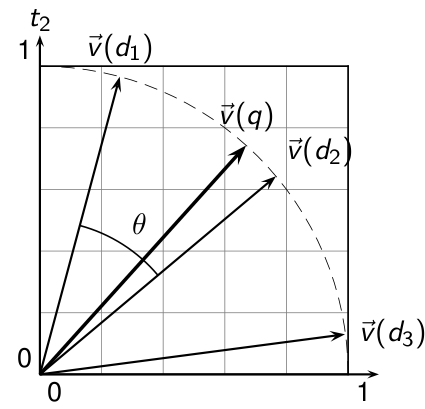
\includegraphics[scale=0.5]{pics/cos.png}
	\caption{ Cosine Similarity.}
\end{figure}

\end{frame}

\begin{frame}{Exercise}
\begin{itemize}
 \item Supongamos que tenemos $3$ documentos, los cuales se forman a partir de las siguientes secuencias de términos: \\
 $d_{1}\rightarrow t_{4}t_{3}t_{1}t_{4}$ \\
 $d_{2}\rightarrow t_{5}t_{4}t_{2}t_{3}t_{5}$ \\
 $d_{3}\rightarrow t_{2}t_{1}t_{4}t_{4}$ \\

\item Construya una matriz término-documento de dimensión $5 \times 3$ usando los pesos $Tf-idf$ simples (sin normalización).
\item Le recomendamos construir primero una lista con la cantidad de documentos en los que aparece cada término (para el idf) 
\item Calcule luego  el $idf$ de cada término.
\item Llene las celdas con los valores $Tf-idf$
\item ¿ A qué documento está más cercano $d_{1}$?
\end{itemize}


\end{frame}

\begin{frame}{Result}
 \begin{table}[htbp]
\caption{Tf-idf Matrix}
\begin{tabular}{|l|r|r|r|}
\hline
 & \multicolumn{1}{l|}{d1} & \multicolumn{1}{l|}{d2} & \multicolumn{1}{l|}{d3} \\ \hline
t1 & 0.176 & 0.000 & 0.176 \\ \hline
t2 & 0.000 & 0.176 & 0.176 \\ \hline
t3 & 0.176 & 0.176 & 0.000 \\ \hline
t4 & 0.000 & 0.000 & 0.000 \\ \hline
t5 & 0.000 & 0.954 & 0.000 \\ \hline
\end{tabular}
\end{table}

\end{frame}

\begin{frame}{Clustering de Documentos [1]}
\footnotesize{
\begin{itemize}
 \item ¿Qué pasa si queremos agrupar los documentos de contenidos similares?
 \item Agrupamos los documentos en conjuntos, donde todos los elementos sean similares entre sí. 
 \item A cada conjunto se le llama  \emph{cluster}. 
 \item El problema de clusterizar, se basa en identificar grupos que maximicen la similitud interna dentro de un cluster y minimicen la similitud entre documentos  pertenecientes a distintos clusters.
\begin{figure}[h!]
	\centering
	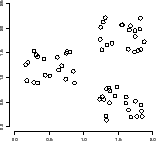
\includegraphics[scale=0.6]{pics/cluster.png}
	\caption{ Conjunto de documentos donde se identifica claramente cada cluster}
\end{figure}
 
\end{itemize}


}
 
\end{frame}

\begin{frame}{Document Clustering [2]}
\footnotesize{
\begin{itemize}
 \item Permite identificar grupos de opiniones similares, o reducir el espacio de búsqueda para una consulta en un buscador. 
 \item K-medias es un algoritmo simple de clustering que requiere la cantidad $k$ de clusters a construir como parámetro.
    \begin{enumerate}
    \footnotesize{
    \item Primero, se identifican aleatoriamente $k$ elementos. Los valores de los atributos de éstos elementos se copian en nuevos elementos llamados centroides de la misma dimensión que éstos. Cada centroide representará un cluster.
    \item Luego se calcula la distancia de todos los $n$ elementos a los $k$ centroides y  se asigna  cada elemento al cluster del centroide más cercano.
    \item Luego se recalcula el valor de los centroides promediando el valor de los atributos de todos los elementos pertenecientes al cluster.
    \item Repite el proceso de calcular las distancias, agrupar los más cercanos y recalcular los centroides hasta que éstos dejen de cambiar. }
    \end{enumerate}

\end{itemize}
}
\end{frame}

\begin{frame}{K-means}
\begin{figure}[h!]
	\centering
	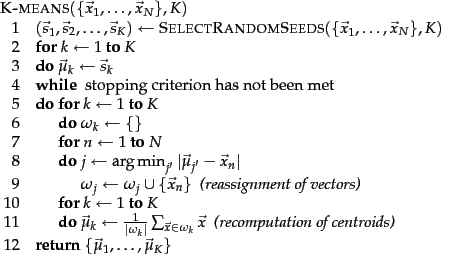
\includegraphics[scale=0.6]{pics/kmeans.png}
	\caption{ K-means algorithm}
\end{figure}


 



 
\end{frame}




\begin{frame}[allowframebreaks]\scriptsize
\frametitle{References}
\bibliography{bio}
\bibliographystyle{apalike}
%\bibliographystyle{flexbib}
\end{frame}



%%%%%%%%%%%%%%%%%%%%%%%%%%%

\end{document}
